\section{w calibration results}
\label{appx:w_calibration}
This section discusses the calibration procedure used to derive a representative value for $w$, the aversion for financial instability from the \citet{suarez2022} welfare function. For any arbitrary value of $w\in(0,\inf)$, it is possible to simulate an optimal policy path $\vec{p}_w$ (see \autoref{fig:arm_policy_simulation_interaction}). Using simple rules, we define 3 preferred policy paths: $\vec{p}_h$, $\vec{p}_b$, and $\vec{p}_c$. The $\vec{p}_h$ path assumes that the historical policy of Armenia is the optimal path. The $\vec{p}_b$ path follows the CCyB rule defined by the Basel Committee \citep{basel2010}, using the credit-to-GDP gap to arrive at optimal values for CCyB. According to estimates performed by \citet{esrb2021}, a “capital-based macroprudential policy corresponds to a CET1 capital of 0.87 of risk-weighted assets.” Using this “conversion rate” we are able to map the CCyB rule to macroprudential policy actions and generate the Basel preferred policy path $\vec{p}_b$. The $\vec{p}_c$ path follows the same logic as $\vec{p}_b$, except for the CCyB values it uses the rule defined by the Czech National Bank (CNB). This rule is defined as a piecewise function that maps different phases of the financial cycle to CCyB decisions \citep{cnb2023}. After applying the “conversion rate” we end up with the policy path $\vec{p}_c$. The historical CCyB policy measures for the Basel and CNB methods are presented in \autoref{fig:arm_ccyb_simulation}.
\begin{figure}
	\centering 
	
\includegraphics[width=0.45\textwidth, angle=0]{Figures/arm_policy_simulation_interaction.png}	
	\caption{Policy path simulation given an arbitrary value for w.} 
	\label{fig:arm_policy_simulation_interaction}%
\end{figure}
\begin{figure}
	\centering 
	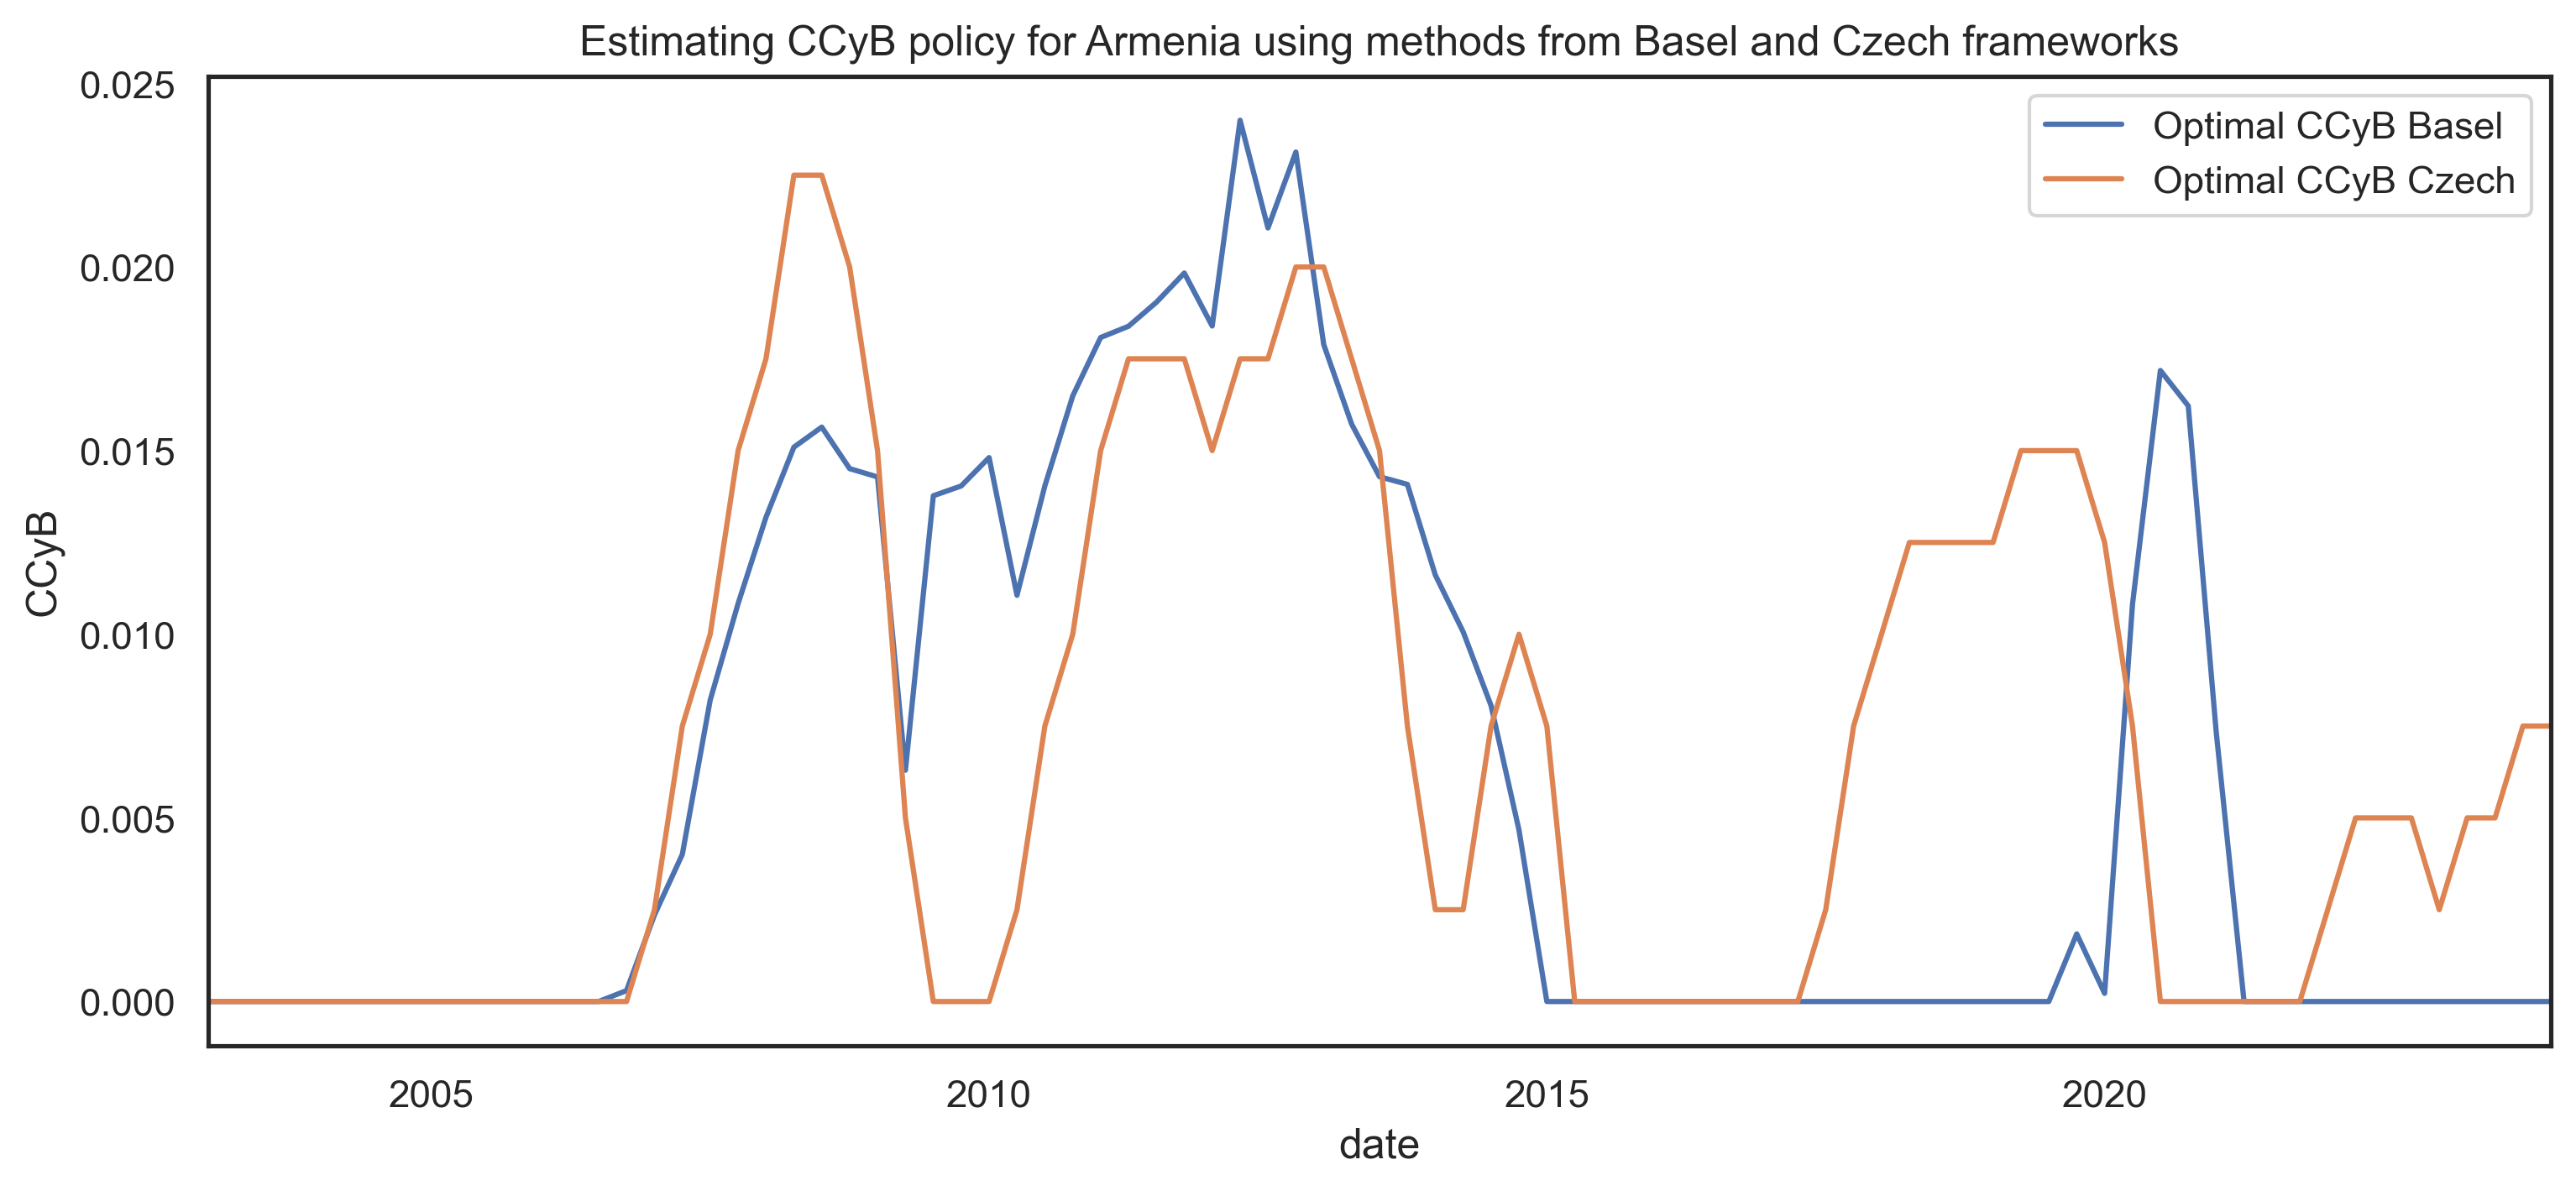
\includegraphics[width=0.45\textwidth, angle=0]{Figures/arm_ccyb_simulation.png}	
	\caption{Optimal CCyB tightening measures derived using the Basel gap and Financial Cycle Index (CNB)} 
	\label{fig:arm_ccyb_simulation}%
\end{figure}

Next, to see which path is the most viable we compare all of the optimal paths $\vec{p}_w$ with the 3 preferred policy paths by taking the Euclidean distance between them. \autoref{fig:arm_w_calibration_interaction} shows the relationship between the choice of $w$ and the 3 preferred policy paths. Using the elbow method and optimal choices from the Basel and CNB methods, we believe that 0.11 is a representative value. This is also equivalent to a relative risk aversion $\rho_0=w\left(\Phi^{-1}(c)\right)^2$ of 3.57, which is in line with the values considered in the literature \citep{cecchetti_2021}.
\begin{figure}
	\centering 
	
\includegraphics[width=0.45\textwidth, angle=0]{Figures/arm_w_calibration_interaction.png}	
	\caption{Euclidean distance between $\vec{p}_w$ and the 3 preferred policy paths for all values of $w$. The dotted lines show the points with the smallest distance.} 
	\label{fig:arm_w_calibration_interaction}%
\end{figure}

As a robustness check for the calibration results above, we ignore the 2 preferred policy paths and instead allow the value of $w$ to change over time. We then select the set $vect{w}$ so that $\vec{p}_{\vec{w}}$ matches almost exactly with $\vec{p}_h$. Finally, we plot the distribution for $w$ in \autoref{fig:arm_w_dynamic_dist}. The selected value of 0.11 is not significantly different from the modes of these distributions.
\begin{figure}
	\centering 
	
\includegraphics[width=0.45\textwidth, angle=0]{Figures/arm_w_dynamic_dist.png}	
	\caption{Distribution for the dynamic values of $w$ over time.} 
	\label{fig:arm_w_dynamic_dist}%
\end{figure}